\section{Fase 6: Modelado y Ejecución}
En esta fase, el científico de datos diseña, crea o utiliza un modelo predictivo o descriptivo y lo alimenta con la versión del conjunto de datos o imágenes obtenidos en la fase de procesamiento y transformación. En esta fase, el científico debe seleccionar el tipo de aprendizaje (supervisado, no supervisado y por refuerzo) y la técnica determinada (regresión, clasificación, clustering, CNN, RNN, etc.) acorde a las preguntas planteadas en el \textit{BCQM}. Hay que mencionar que en esta fase el \textit{Data Analysis Team} debe definir junto al medico experto en oncología la tolerancia de error permitida en el modelo, esto dado a que la sensibilidad de los análisis puede variar dependiendo del tipo de cáncer de mama y la técnica de diagnostico. Es probable que el científico de datos pruebe múltiples algoritmos con sus respectivos parámetros para encontrar el mejor modelo para las variables oncológicas disponibles. Cabe resaltar, que es de vital importancia que los modelos propuestos no tengan problemas de sobre-ajuste o infra-ajuste ya que esto puede generar resultados erróneos o poco significativos. Adicionalmente, el científico de datos en cuestión junto al \textit{Data Analysis Team} deben definir la infraestructura a nivel de servidor necesaria para el entrenamiento y prueba del modelo según la cantidad de información a procesar, esto con el proposito de generar resultados acertados en el menor tiempo posible en pro de cumplir las tareas definidas en la fase de planeación de actividades y dar valor a los datos oncológicos una vez finalice el \textit{Release}.

\subsection{Agrupamiento(Clustering)}

\begin{table*} [!htb]
	\footnotesize
	\begin{threeparttable}
		\caption{Modelos Machine Learning para agrupamiento (Clustering).}
		\label{Clustering_Models}
		\begin{tabular}{p{2cm} p{4cm} p{9cm}} \toprule	
		\begin{center}ID\end{center}   
		&\begin{center}Nombre\end{center}             
		&\begin{center}Librería\end{center}      
		\\ \hline kmeans & K-Means Clustering & sklearn.cluster.\_kmeans.KMeans
		\\ \hline ap & Affinity Propagation & sklearn.cluster.\_affinity\_propagation.AffinityPropagation
		\\ \hline meanshift & Mean Shift Clustering & sklearn.cluster.\_mean\_shift.MeanShift
		\\ \hline sc & Spectral Clustering & sklearn.cluster.\_spectral.SpectralClustering
		\\ \hline hclust & Agglomerative Clustering & sklearn.cluster.\_agglomerative.AgglomerativeClustering
		\\ \hline dbscan & Density-Based Spatial Clustering & sklearn.cluster.\_dbscan.DBSCAN
		\\ \hline optics & OPTICS Clustering & sklearn.cluster.\_optics.OPTICS
		\\ \hline birch & Birch Clustering & sklearn.cluster.\_birch.Birch
		\\ \hline kmodes & K-Modes Clustering & kmodes.kmodes.KModes
		\\ \hline
		\end{tabular}
	\end{threeparttable}
\end{table*}


\begin{figure}
	\setlength\tabcolsep{3pt}%%
	\centering
	\begin{tabular}{ccc}
		\textbf{K-Means} &
		\textbf{Affinity Propagation} \\
		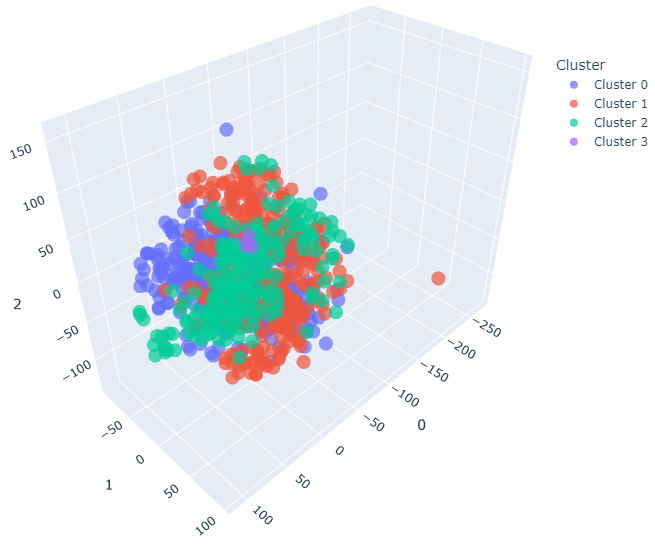
\includegraphics[width=0.5\textwidth]{NOTEBOOK/IMAGENES_CLUSTERING/TNSE_Kmeans} &
		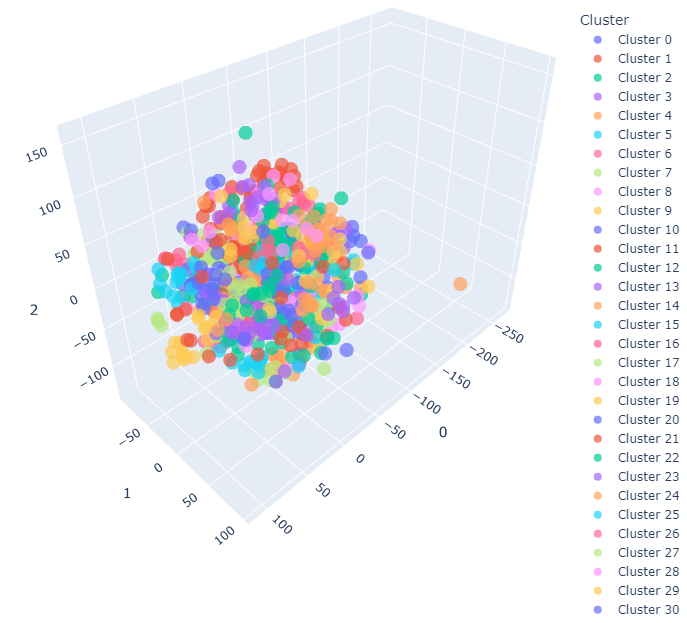
\includegraphics[width=0.5\textwidth]{NOTEBOOK/IMAGENES_CLUSTERING/TNSE_Affinity_Propagation} \\
		
		\textbf{Mean Shift Clustering} &
		\textbf{Spectral Clustering} \\
		
		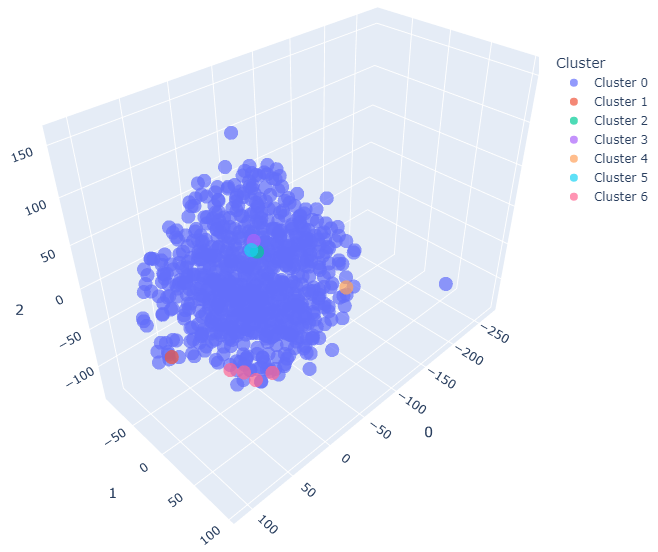
\includegraphics[width=0.5\textwidth]{NOTEBOOK/IMAGENES_CLUSTERING/TNSE_Mean_Shift_Clustering} &
		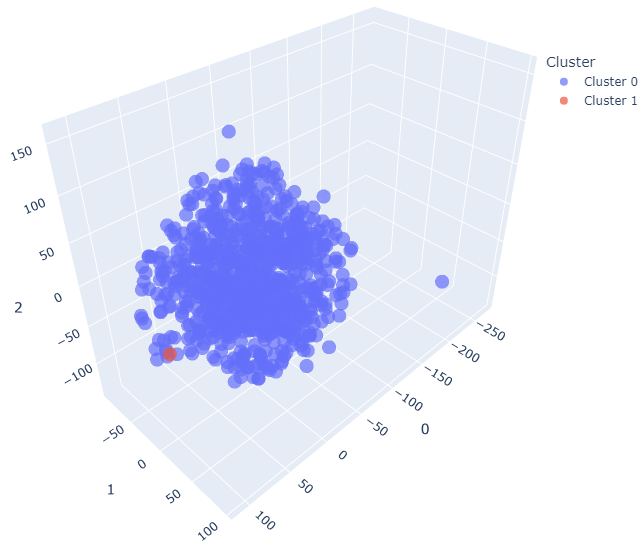
\includegraphics[width=0.5\textwidth]{NOTEBOOK/IMAGENES_CLUSTERING/TNSE_Spectral_ Clustering} \\ 
		
		\textbf{Agglomerative Clustering} &
		\textbf{Density-Based Spatial Clustering} \\
		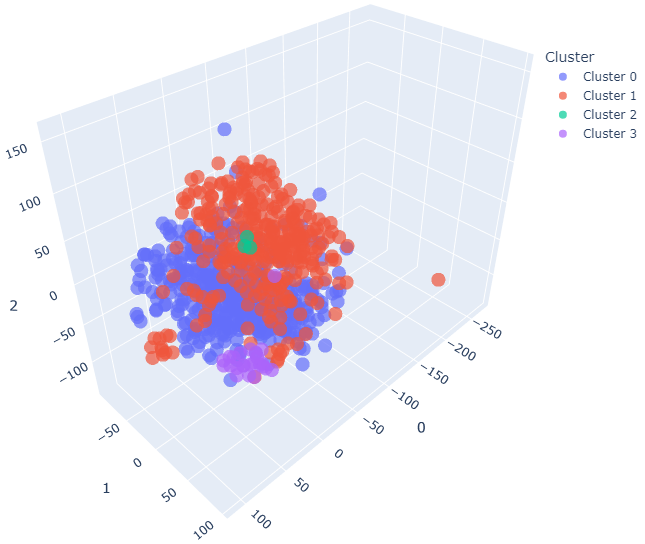
\includegraphics[width=0.5\textwidth]{NOTEBOOK/IMAGENES_CLUSTERING/TNSE_Agglomerative_Clustering} &
		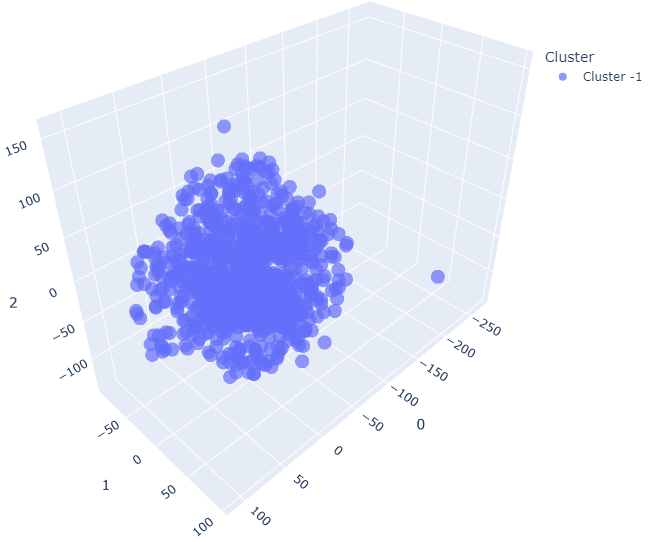
\includegraphics[width=0.5\textwidth]{NOTEBOOK/IMAGENES_CLUSTERING/TNSE_Density_Based_Spatial_Clustering} 
	\end{tabular}
\end{figure}

\begin{figure}
	\setlength\tabcolsep{3pt}%%
	\centering
	\begin{tabular}{ccc}
		\textbf{OPTICS Clustering} &
		\textbf{Birch Clustering} \\
		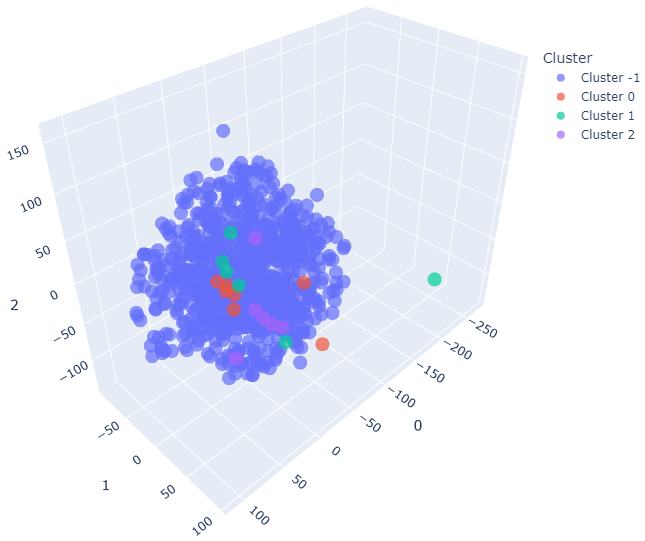
\includegraphics[width=0.5\textwidth]{NOTEBOOK/IMAGENES_CLUSTERING/TNSE_OPTICS Clustering} &
		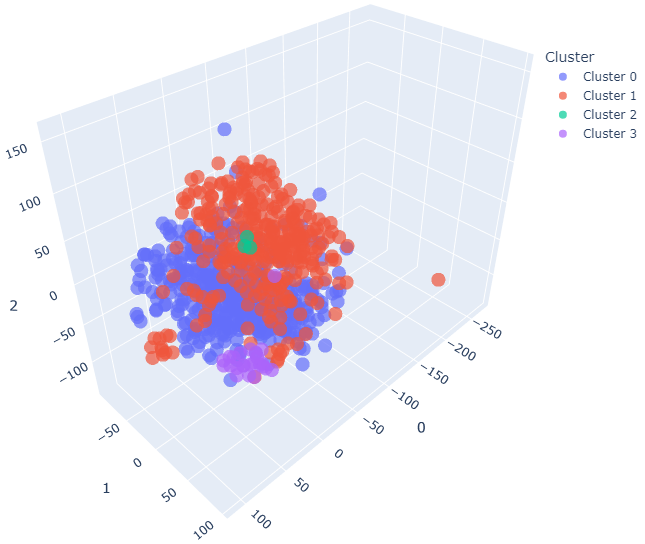
\includegraphics[width=0.5\textwidth]{NOTEBOOK/IMAGENES_CLUSTERING/TNSE_Agglomerative_Clustering} 
	\end{tabular}
\end{figure}

\begin{figure}
	\setlength\tabcolsep{3pt}%%
	\centering
	\begin{tabular}{c}
		\textbf{K-Modes Clustering} \\
		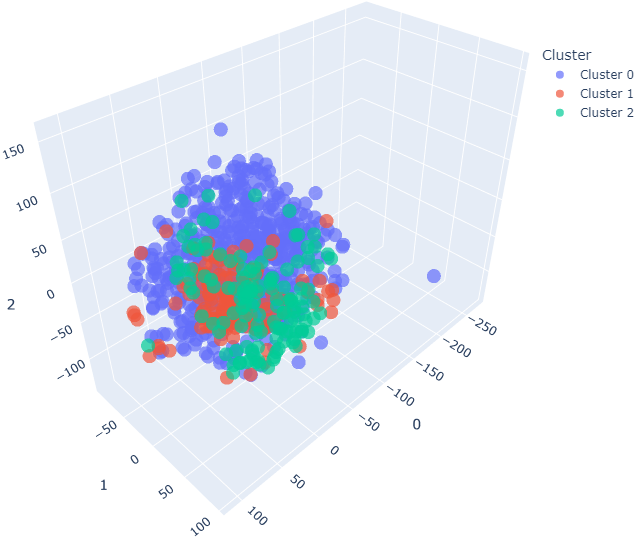
\includegraphics[width=0.5\textwidth]{NOTEBOOK/IMAGENES_CLUSTERING/TNSE_Kmodes}
	\end{tabular}
	\caption{Modelos Clustering aplicados al conjunto de datos del Carcinoma invasivo de mama (TCGA, Cell 2015). }
	\label{Clustering_Models_graphics}
\end{figure}


 

\subsection{Clasificación Multiclase}

